\section{\tool: UI Analysis Tool}
\label{sec:integriTool}

Our labeling scheme helps web service developers to prevent swapping attacks. An obvious approach for developers is to require that users label all inputs. However, as labeling increases user effort, a better approach is to ask the user to label only those input fields that are interchangeable and thus susceptible to swapping. In this section, we describe a UI analysis tool, called \tool, that helps developers to identify input fields that should be protected. When developers request labeling for those fields only, our tool also reduces user effort.

\begin{figure}[t]
 \centering
 %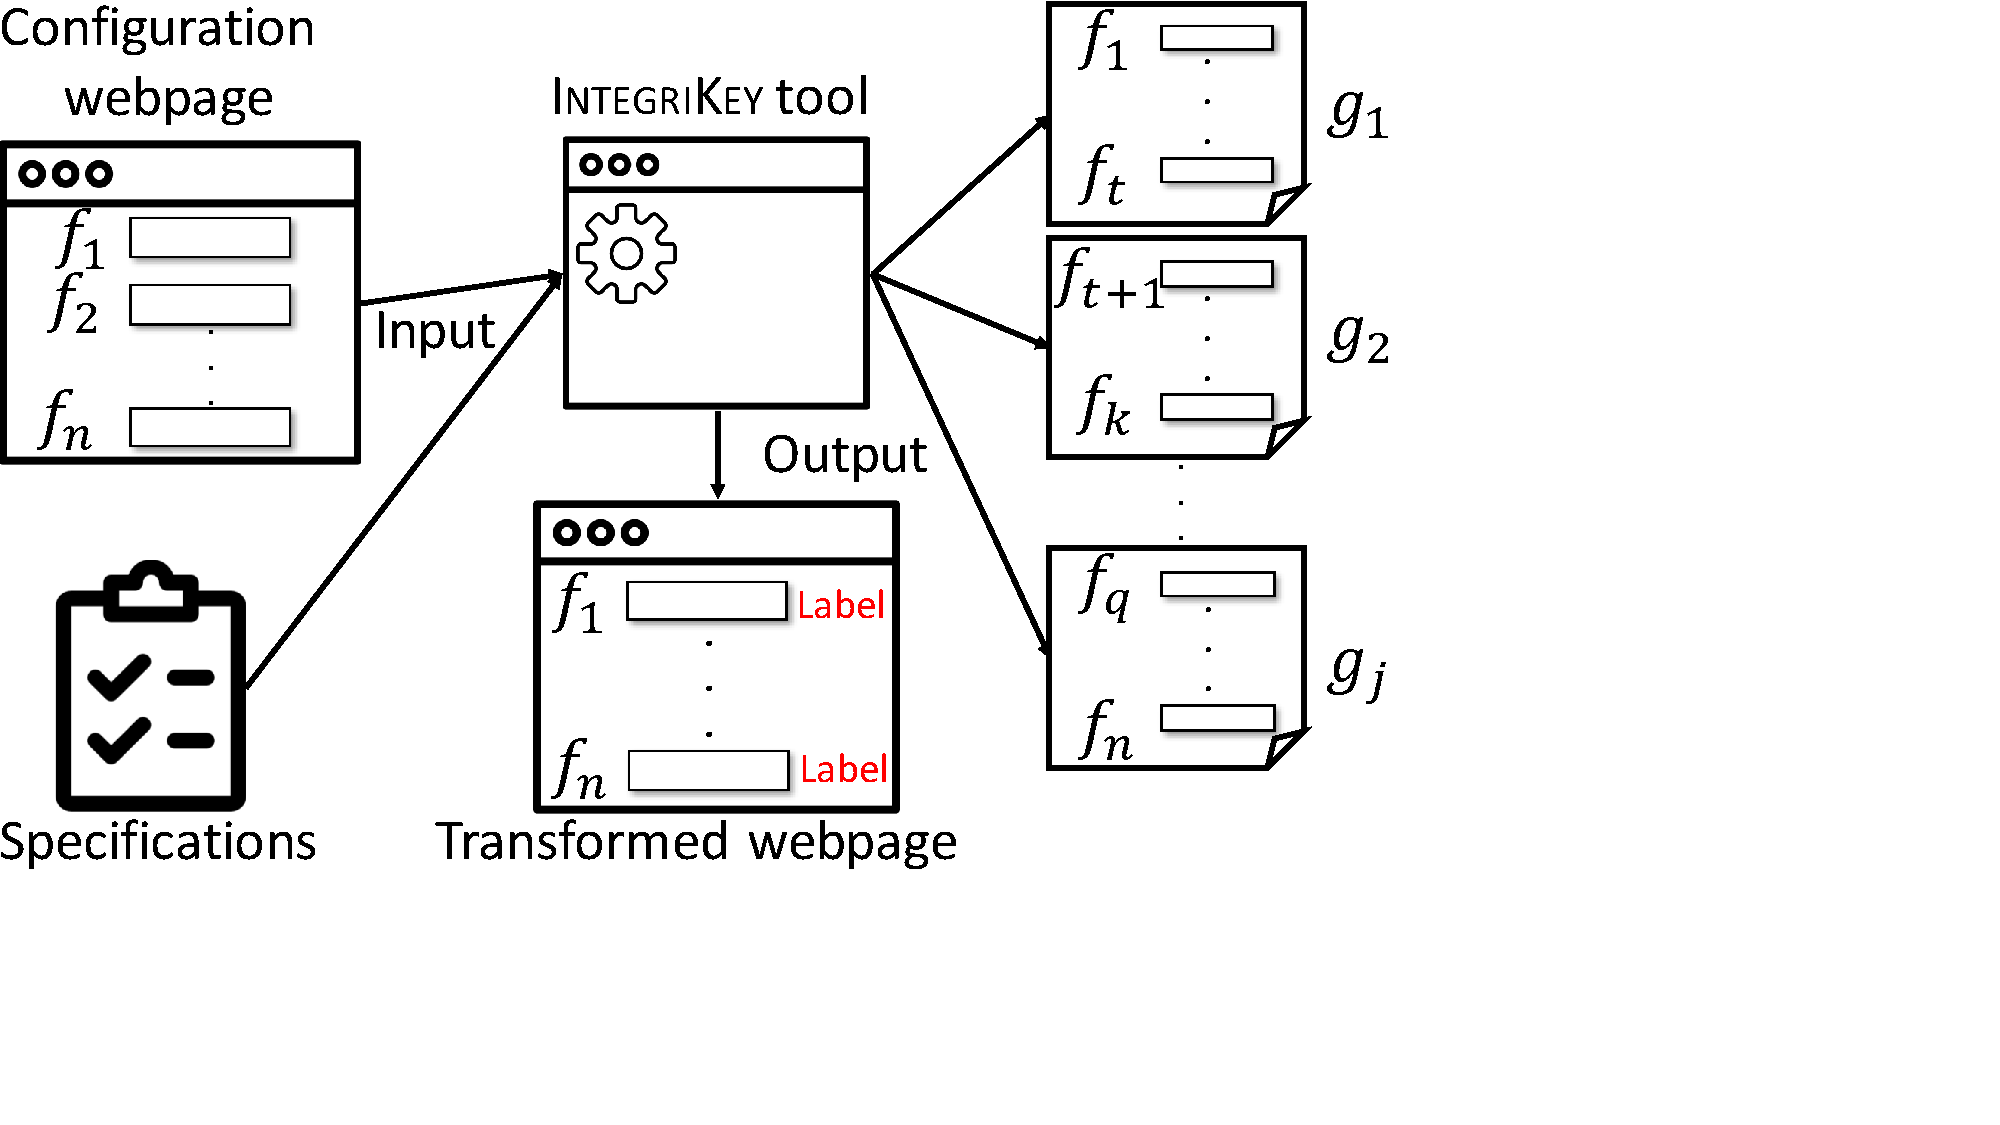
\includegraphics[trim={0 4cm 9cm 0},clip,width=\linewidth]{ServerSideTool_revised_1.pdf}
 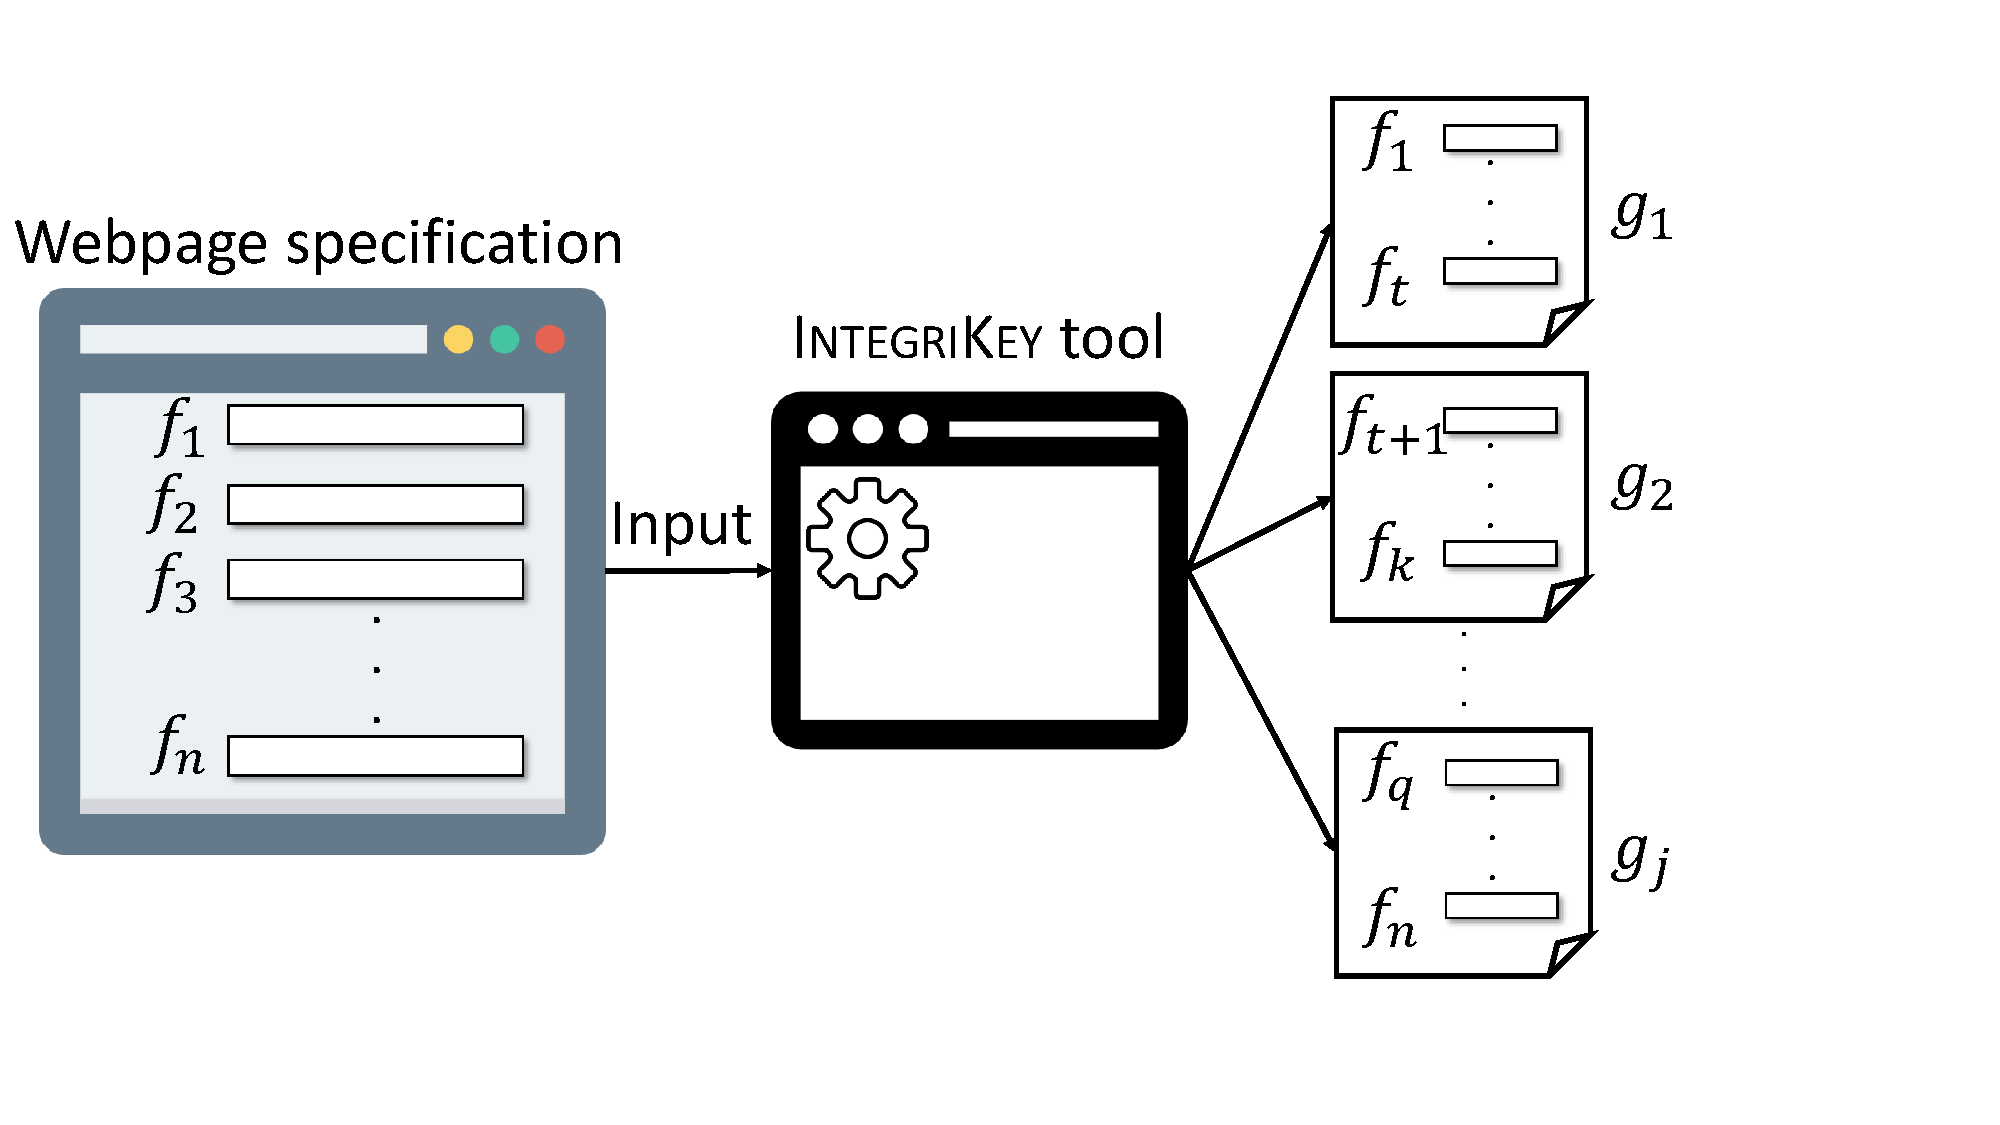
\includegraphics[trim={0 2.3cm 12cm 0},clip,width=0.6\linewidth]{chapters/IntegriKey/images/ServerSideTool.pdf}
 \caption[\tool overview]{\textbf{\tool overview}. \tool takes a web page (HTML file) and a web page specification with input fields $f_1, f_2, f_3$. In this example $f_1$ and $f_2$ are swappable. The final output is a transformed webpage with labelling information ($f_1$ and $f_2$ requires labelling) for the users and converted mouse based UIs (drop-down menus, radio buttons, sliders etc.) to text fields. 
 %Example screenshot of transformed webpage is illustrated in Figure~\ref{fig:labelEx}.
 }
 %\vspace{-10pt}
 \label{fig:tool}
\end{figure}

Figure~\ref{fig:tool} illustrates an overview of the tool that takes two inputs. The first input is the HTML code of the web form. The second input is a user interface specification that contains definitions for all input fields in the page. \tool processes the provided inputs and outputs a generated webpage which is annotated with labeling instructions for the user. For example, for a user interface with input fields $f_1, f_2, f_3$ where $f_1$ and $f_2$ are interchangeable, the tool outputs a webpage with the labelling instruction for $f_1$ and $f_2$. An example screenshot of a webpage generated using our tool is shown in Figure~\ref{fig:labelEx}.
 

\subsection{UI Specification} 
\label{sec:integriTool:specification}

The UI specification needs to be manually written by the developer. The specification captures the fact whether two user input fields in the UI are interchangeable. One such example is a home automation system, where the user can set the temperature of a specific room by providing the input to the web application. The attacker can swap input fields for temperatures of two rooms. Another and more interesting example is a UI where two fields are semantically different but share the similar format. Consider, for example, the configuration of a medical device, where the doctor can set blood pressure and heart rate limit. As the range of these two fields is overlapping, the attacker can swap the two fields even though they are semantically very different.

\lstset{language=XML, frame=tb, caption=\textbf{A webpage specification example.} This web page specification corresponds to our running user interface example that is illustrated in Figure~\ref{fig:swapExample}., label = snippet:specificationXML, firstnumber =1}
\begin{figure}[t]
\begin{lstlisting}[mathescape=true]
<InputSchema>
 <Input>
   <ID>Relay 1</ID>
   <Format>s[a-zA-Z0-9]+[min=1,max>min]</Format></Input>
 <Input>
   <ID>Decimal places 1</ID>
   <Format>i[0-9]*[min=0,max=5]</Format></Input>
 <Input>
   <ID>Type 1</ID>
   <Format>m[{int, float, bool}]</Format></Input>
 <Input>
   <ID>Relay temp 1</ID>
   <Format>i[0-9]*[min=-20,max=150]</Format></Input>
 <Input>
   <ID>Relay 2</ID>
   <Format>s[a-zA-Z0-9]+[min=1,max>min]</Format></Input>
 <Input>
   <ID>Decimal places 2</ID>
   <Format>i[0-9]*[min=0,max=5]</Format></Input>
  <Input>
   <ID>Type 2</ID>
   <Format>m[{int, float, bool}]</Format></Input>
 <Input>
   <ID>Relay temp 2</ID>
   <Format>i[0-9]*[min=-10,max=100]</Format></Input>
 <Input>
   <ID>Unit</ID>
   <Format>s[unit][min=1, max=5]</Format></Input>
</InputSchema>
\end{lstlisting} 
%\vspace{-5pt}
\end{figure}

The user interface specification is an XML document that defines each user input field. Specification~\ref{snippet:specificationXML} shows an example for our running example UI. For each user input field, the specification provides the identifier of the web form element and its format. The format defines the type of the input (e.g., string (\texttt{s}) or integer (\texttt{i})) and constraints for the acceptable value (e.g., a regular expression for a string or the minimum and maximum values for an integer).
More precisely, we define the input format as:%\vspace{-8pt}

$$type[regx][min = x, max = y][\{elements\}]^*$$
%
where $type$ denotes the input field data type such as \String($s$), \integer($i$), \float($f$), \Date($d$), \Time($t$), \menu($m$) and \radio ($r$). $[regx]$ defines the regular expression for acceptable values. $min$ and $max$ define possible minimum and maximum \String length or minimum and maximum values if the type is \integer, \float, \Date or \Time. The optional $[\{elements\}]$ is only applicable to UI objects such as \Menu (such as drop down menus) and \radio. $\{elements\}$ represents all the objects in the given UI element that can be chosen by the user.  


We note that \tool requires a tight specification to provide a precise output. If the developer provides a coarse-grained specification, that leads to an over-approximation of swappable fields by the tool that increases user effort but will not impose security risk.

\subsection{Tool Processing} 

\tool processes all input fields from the specification by evaluating them based on their specification. For numeric input fields (\integer, \float, \Time, \Date) the test checks for overlapping acceptable values, i.e., a boundary condition test. %Let $f_i^{max}$ and $f_i^{min}$ denote the maximum and minimum values for field $f_i$. If either of the following conditions hold: $f_i^{max} < f_j^{min} \ \text{or}\ f_i^{min} > f_j^{max}$ then there exist no values that are the valid inputs to $f_i$ and $f_j$ at the same time. 
%
For \String fields, our tool tests if the format constraints of two input fields can be met at the same time. For example, consider the following expressions:\vspace{2pt}
\begin{align*}
RE_1 &= s[a-zA-Z]^+[min=x, max=y]\\
RE_2 &= s[a-zA-Z0-9]^+[min=x, max=y]\\
&\implies RE_1 \subsetneq  RE_2
\end{align*}
where $RE_1$ represents a \String containing uppercase or lowercase alphabetic characters and $RE_2$ represents a \String containing uppercase or lowercase alphabetic or numerical characters. In this case, $RE_1$ is a subset of $RE_2$ as all strings from $RE_1$ are also members of $RE_2$ but there are strings in $RE_2$ that are not in $RE_1$. This can be verified by checking if $RE_1\cap (RE_2)^c = \phi \implies RE_1 \subset RE_2$, where $\phi$ denotes empty set.
%
In general, two fields $f_i$ (corresponding regular expression $RE_i$) and $f_j$ (corresponding regular expression $RE_j$) can be swapped  if and only if $RE_i \cap RE_j \neq \phi$ and, $f_i$ \& $f_j$ shares at least two elements. A short proof for this is as the following:

\begin{proof}
  Let $F_x$ and $F_y$ be two input fields and their corresponding regular expressions are $RE_x$ and $RE_y$. If $F_x$ and $F_y$ are swappable fields, then $RE_x$ and $RE_y$ have at least two overlapping accepted input.
  \\
  If $F_x$ and $F_y$ are swappable, then 
  $$\exists x_i \in RE_x : x_i \in RE_y\ \text{and}\ \exists y_j \in RE_y : y_j \in RE_x$$ 
  This was the input values $x_i$ and $y_j$ can be swapped.
  Hence, $\{x_i, y_j\} \in RE_x \cap RE_y \Rightarrow |RE_x \cap RE_y| \geq 2$ 
\end{proof}

\begin{algorithm}[!htpb]
\footnotesize
\DontPrintSemicolon
\KwIn{Specification $S$ with input fields $F$.}
\KwOut{Set of subset of fields $G=\{g_1,\ldots,g_n\}$ where all the fields in a $g_i\in G$ are swappable.}
%\Begin
%{
    $G\leftarrow$ Initialize empty group\\
    \For{$\forall f \in F$} {
        \For{$\forall f_{in} \in F$} {
            %\If{$f \neq f_{in} \wedge f.type = f_{in},type$} {
                %$addField \leftarrow false$\\         
                $f.regEx, f_{in}.regEx \leftarrow$ read from $S$\\        
                \If{$f.type = $ \texttt{string}} {       
                    \lIf{$f.regEx \subset f_{in}.regEx$} {  \label{algo:makeGroup:regEx}   
                        $addField \leftarrow true$ 
                     }
                     \If{$f_{in}.type = (\menu\ \vee \radio$)} { 
                            \lIf{$f_{in}.elements \in f.regEx$} { \label{algo:makeGroup:member} 
                             $addField \leftarrow true$ 
                         }
                     }  
                }
                \If{$f.type=(\texttt{integer} \vee \texttt{float} \vee \texttt{time} \vee \texttt{date})$} {
                    \If{$f_{in}.type=(\menu \vee \radio)$} {\label{algo:makeGroup:menuNum} 
                    
                        $f_{in}^{min} \leftarrow min(f_{in}.elements)$\\
                        $f_{in}^{max} \leftarrow max(f_{in}.elements)$\\
                    }
                    \lIf{$\lnot(f^{max} < f_{in}^{min} \vee f^{min} > f_{in}^{max})$}{ \label{algo:makeGroup:numCheck}
                        $addField \leftarrow true$  
                    }
                    
                }
                \If{$f.type = $ (\texttt{menu} $\vee$ \texttt{radio button}) $\wedge f_{in}.type = $ (\texttt{menu} $\vee$ \texttt{radio button})}{ \label{algo:makeGroup:intersection}
                    \lIf{$f.elements \cap f_{in}.elements \neq \phi$}
                    {
                        $addField \leftarrow true$      
                    }
                }
                
                \If{$addField = true$}{
                    $g \leftarrow$ empty set of fields\\
                    $g.add(f, f_{in})$\\
                    $G.add(g)$\\
                    $addField \leftarrow false$
                %}
                }
        }
    }
    return $G$
%}
\caption{\small{This algorithm finds swappable user input fields based on user interface specification.}} 
\label{algo:makeGroup}
\end{algorithm}
%\vspace{-10pt}

Based on such tests, we design Algorithm~\ref{algo:makeGroup} that generates a group of overlapping input fields. The algorithm works by \emph{comparing every user input field to all the other fields} in the specification.

If one of the two compared fields is \String and another is \string or number (\integer, \float, \Date and \Time) type, we check if their regular expression if overlapping (line~\ref{algo:makeGroup:regEx}). If one of the fields is \String and another is either \menu or \radio, then we check if an element of the \menu (or \radio) is a member of the \String regular expression (line~\ref{algo:makeGroup:member}). 
%
If both of the compared fields are of the numeric type, then we check for the boundary condition (line~\ref{algo:makeGroup:numCheck}). The boundary check is also done for the elements of \menu and \radio as the members could be number type (line~\ref{algo:makeGroup:menuNum}).
If both fields are \menu or \radio type, then we check if the intersection of two fields is empty (line~\ref{algo:makeGroup:intersection}).

Evaluating if a regular expression is a subset of another requires conversion of the regular expression to a deterministic finite automaton (DFA). The algorithm requires computing pairwise swappable tests over all the fields in the specification and returns groups of swappable fields. We analyze the complexity and performance of this algorithm in Section~\ref{sec:results}.


\myparagraph{UI conversion} For drop-down menu and radio button inputs, our tool simply checks for overlapping \Menu and \radio elements. Our tool converts such elements into the corresponding textual representation to enable form completion with the keyboard. This is illustrated in Figure~\ref{fig:uiConv}, where an example \radio with two options (\texttt{on} or \texttt{off}) is replaced with a textfield where the user is asked to type in either value \texttt{on} or \texttt{off}, correspondingly. Similarly, drop-down menus and slider elements are converted to a text input fields. 

\begin{figure}[t]
 \centering
  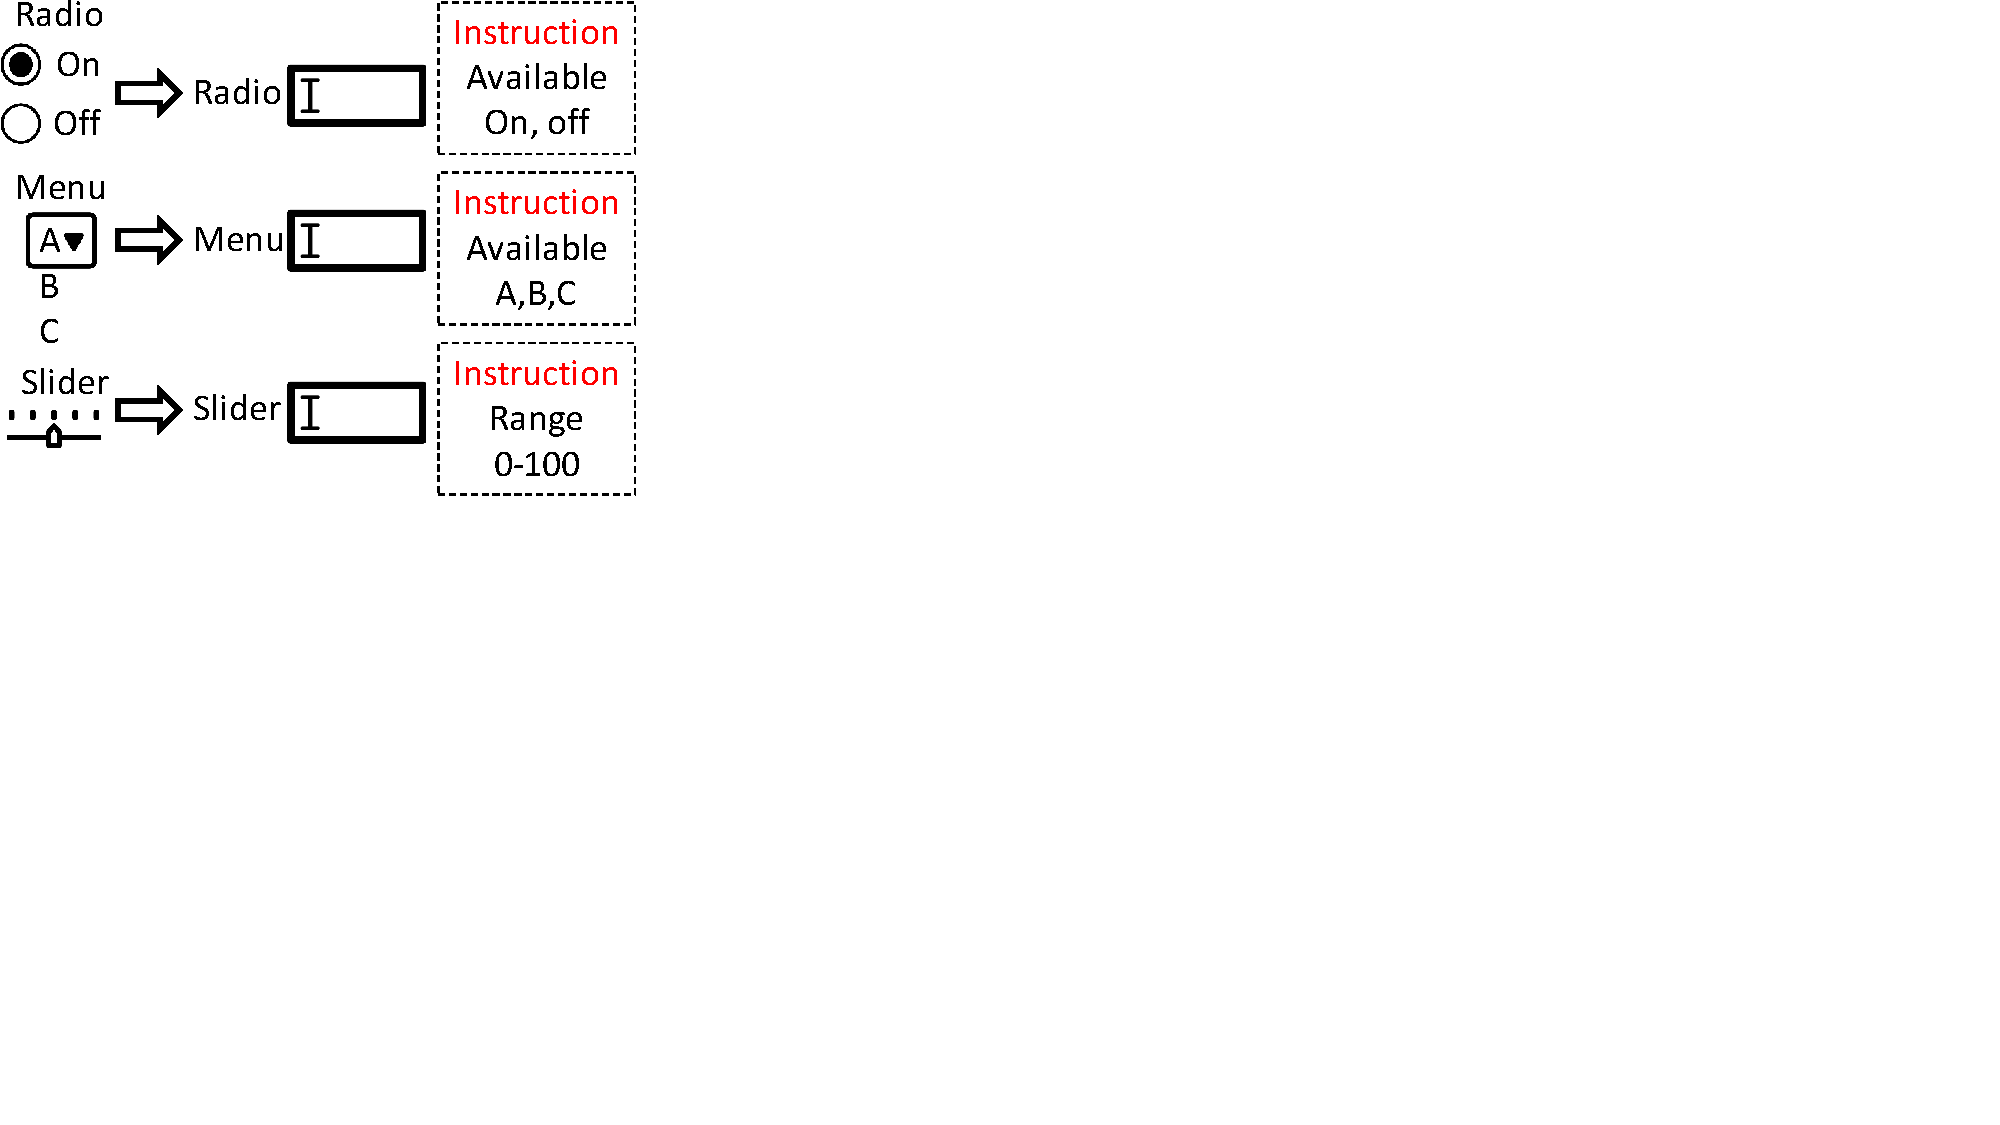
\includegraphics[trim={0 9cm 23cm 0},clip,width=0.5\linewidth]{chapters/IntegriKey/images/UIConvert.pdf}
 \caption[UI conversion]{\textbf{UI conversion.} Conversion of radio button, drop-down menu and slider to an equivalent text field with added instructions.}
 \vspace{-10pt}
 \label{fig:uiConv}
\end{figure}


\subsection{Web Page Annotation} 

The second output of \tool is an annotated user interface. Our tool generates labeling instructions for users and embeds them into the web form, i.e., our tool instruments the HTML code. The instruction includes what label the user should add before each input value. 

For choosing label names, we implement a simple approach, where \tool takes the first three characters from each of the words. For example \texttt{'Relay temp 1'} converts to \texttt{'reltem1'}. Other label generation approaches are, of course, possible as well. In case of collision of generated labels, \tool appends an incremented counter at the end of the label. Additionally, if there are multiple configuration pages (web forms) on the remote server that are identical, \tool also appends an incremented counter. This ensures that no two text fields have identical labels. 

An example of the tool's output is shown in Figure~\ref{fig:labelEx} which was produced using our running example UI and the specification listed in Specification~\ref{snippet:specificationXML} as inputs. 
%The example shows the group of overlapping fields, the annotation and transformed UI elements (drop-down menus to the text field). 

%\myparagraph{Example.} Tool takes the specification provided in  Specification~\ref{snippet:specificationXML} and produces two groups:  $g_1=$\{\texttt{Relay 1, Relay 2}\} and $g_2$ =\{\texttt{Temp Relay 1, Temp Relay 2, Decimal places 1, Decimal places 2}\} that are overlapping set of fields while the \texttt{Unit} field is distinct from the rest. Note that the precise calculation of the overlapping groups of fields requires the developer to provide a tight/well-defined specification otherwise, the tool may over-approximate.

